\documentclass{article}

% --- packages ---
\usepackage[utf8]{inputenc}
\usepackage[T1]{fontenc}
\usepackage{amsmath,amssymb,amsfonts,amsthm}
\usepackage{graphicx}
\usepackage{booktabs}
\usepackage{hyperref}
\usepackage{float}
\usepackage{xcolor}
\usepackage[margin=1in]{geometry}
\usepackage{natbib}
\usepackage{subcaption}
\usepackage{tikz}
\usepackage{pgfplots}
\pgfplotsset{compat=1.17}
\usetikzlibrary{positioning,arrows.meta,calc,fit,backgrounds,shapes.geometric}

% --- theorem environments ---
\newtheorem{definition}{Definition}
\newtheorem{proposition}{Proposition}
\newtheorem{remark}{Remark}

% --- macros ---
\newcommand{\R}{\mathbb{R}}
\newcommand{\E}{\mathbb{E}}
\newcommand{\model}{\textsc{BF-ConvUNeXt}}
\newcommand{\convnext}{\textsc{ConvNeXt}}
\newcommand{\bfbn}{\textsc{BiasFreeBatchNorm}}
\newcommand{\sigpx}{\sigma_{255}}

% --- colors for charts ---
\definecolor{oursblue}{RGB}{31,119,180}
\definecolor{classicgray}{RGB}{127,127,127}
\definecolor{sotaorange}{RGB}{255,127,14}
\definecolor{gaborgreen}{RGB}{44,160,44}
\definecolor{skipred}{RGB}{214,39,40}
\definecolor{bottlepurple}{RGB}{148,103,189}

\title{A Compact Bias-Free ConvNeXt U-Net for Blind Gaussian Image Denoising\\
\large{Frozen Gabor stem, Laplacian-pyramid skips, and end-to-end degree-1 homogeneity, evaluated against the color-denoising leaderboard}}

\author{
  Nikolas Markou \\
  \texttt{nikolasmarkou@gmail.com}
}

\date{}

\begin{document}

\maketitle

% ============================================================================
\begin{abstract}
We describe and evaluate \model{}, a compact bias-free \convnext{} U-Net for blind additive-white-Gaussian-noise (AWGN) image denoising. The network is an \emph{integration} of four ingredients, none individually novel: a frozen depthwise \textbf{Gabor stem} (an oriented band-pass front end that contributes zero trainable parameters), a \textbf{Laplacian-pyramid} encoder that routes the full-resolution high-frequency residual into the skip connection (with three extra \convnext{} blocks per skip band), a \textbf{\convnext{}-V1 U-Net} body, and \textbf{end-to-end bias-freedom} --- every convolution has no additive bias, the head is linear, activations are LeakyReLU, and normalization is a variance-only batch norm --- so that the whole $3.39$M-parameter network is exactly degree-1 homogeneous, $D(\alpha y)=\alpha D(y)$, at inference. Homogeneity is the structural property that licenses the Miyasawa/Tweedie reading of the denoiser residual as a (scaled) score, and, following Mohan et al., underwrites blind generalization across noise levels from a single model. We train one blind model with a linear noise-$\sigma$ curriculum spanning $\sigpx\!\approx\!6$--$127$ and evaluate it, unchanged, against the published color-denoising leaderboard on all four standard sets (CBSD68, Kodak24, McMaster, Urban100) at $\sigma\!\in\!\{15,25,50\}$ under the full-image protocol. The single blind model \textbf{beats DnCNN and FFDNet on every set at every noise level} (average $+0.7$\,dB over DnCNN; FFDNet is non-blind yet still trails), and sits a small, consistent margin behind the heavyweight CNN/transformer state of the art --- $\sim\!0.4$\,dB on CBSD68/Kodak24, $\sim\!0.7$\,dB on McMaster, $\sim\!1.0$\,dB on Urban100 --- at roughly one tenth of their parameters. We are deliberately honest about what bias-freedom does \emph{not} buy: the homogeneity is inference-only and checkpoint-specific, and the learned residual field is measurably non-conservative, so no global prior/energy exists and plug-and-play/RED convergence or calibrated-uncertainty guarantees do not transfer. We report PSNR only, on a single checkpoint, without ablations; those are stated as future work rather than glossed over.
\end{abstract}

% ============================================================================
\section{Introduction}
\label{sec:intro}

Blind Gaussian image denoising --- recovering a clean image $x$ from $y = x + \varepsilon$, $\varepsilon \sim \mathcal{N}(0,\sigma^2 I)$, with $\sigma$ \emph{unknown at test time} --- is both a canonical low-level vision task and a workhorse module inside modern inverse-problem solvers. Two facts frame this paper. First, the field's accuracy is dominated by large transformer/CNN hybrids (DRUNet, SwinIR, Restormer, SCUNet) with tens of millions of parameters, often trained per-noise-level. Second, a much older and simpler observation --- that removing \emph{all} additive constants from a denoising CNN makes it exactly scale-equivariant and hence able to generalize blindly across noise levels a biased network cannot handle \citep{mohan2020biasfree} --- remains underexploited in a modern architecture.

This paper takes the second fact seriously and asks a narrow, empirical question: \emph{how far does a deliberately compact, strictly bias-free, modern-conv-block U-Net get on the standard color-denoising leaderboard, as a single blind model?} Our answer is \model{}, a $3.39$M-parameter bias-free \convnext{} U-Net that composes four ideas we did not invent:

\begin{itemize}
  \item a \textbf{frozen depthwise Gabor stem} \citep{gabor1946} --- a bank of oriented, frequency-tuned band-pass filters fixed at initialization (zero trainable parameters), followed by a single learned $1{\times}1$ mixing projection;
  \item a \textbf{Laplacian-pyramid encoder} \citep{burt1983laplacian} that, at each downsampling junction, sends the full-resolution high-frequency residual band to the skip connection and passes the low-frequency band downward, with three extra \convnext{} blocks applied to each high-frequency skip band;
  \item a \textbf{\convnext{}-V1 U-Net} \citep{liu2022convnext,ronneberger2015unet} body (depthwise $7{\times}7$ conv, inverted-bottleneck MLP, LayerScale);
  \item \textbf{end-to-end bias-freedom}: no additive bias in any layer, a linear head, LeakyReLU activations, and a variance-only batch normalization, chosen jointly so the network is globally degree-1 homogeneous at inference.
\end{itemize}

The scientific content is not that any of these pieces is new; it is (a) the specific, carefully bias-preserving way they are combined so that homogeneity survives end-to-end, and (b) an honest, apples-to-apples measurement of the result against the published leaderboard using the same test sets and full-image protocol. The headline is favorable: the compact blind model uniformly beats the classic sub-1M CNNs and lands about half a dB behind models an order of magnitude larger.

\subsection{What this paper is (and is not)}
\label{sec:scope}

This is an \emph{integration-and-evaluation} paper in the register of an engineering report, not a novel-component paper. Specifically:

\begin{enumerate}
  \item We contribute a precise description of \model{} --- the exact topology, the frozen Gabor stem, the Laplacian-pyramid skip decomposition, the \convnext{}-V1 block, and the bias-free construction that makes the whole network degree-1 homogeneous --- at a level of detail sufficient to reimplement it.
  \item We contribute a fair benchmark: one blind checkpoint, evaluated unchanged on all four standard color sets at three noise levels under the full-image protocol, tabulated against six published baselines.
  \item We are explicit about the theory's \emph{limits}: the Miyasawa/Tweedie residual-as-score reading is a motivation, and we show (Section~\ref{sec:limitations}) that the learned operator is non-conservative, so it is \emph{not} the gradient of any global prior.
\end{enumerate}

What this paper is \emph{not}: it is not a claim that Gabor stems, Laplacian skips, \convnext{} blocks, or bias-free CNNs are new; it is not an ablation study (we do not isolate each component's contribution here --- see Section~\ref{sec:limitations}); it reports \textbf{PSNR only} (SSIM was not measured); and it makes \textbf{no claim} of a calibrated prior, an exact likelihood, or plug-and-play convergence guarantees. We would rather under-claim on a single honest checkpoint than over-claim.

% ============================================================================
\section{Architecture}
\label{sec:arch}

\model{} is a two-level U-Net operating on images normalized to $[-0.5, +0.5]$. All parameter counts and layer shapes below are read from the actual trained checkpoint (\texttt{convunext\_denoiser\_base}, $3{,}393{,}936$ parameters total: $3{,}378{,}540$ trainable and $15{,}396$ frozen). Figure~\ref{fig:arch} shows the data flow.

\begin{figure}[H]
\centering
\resizebox{\textwidth}{!}{%
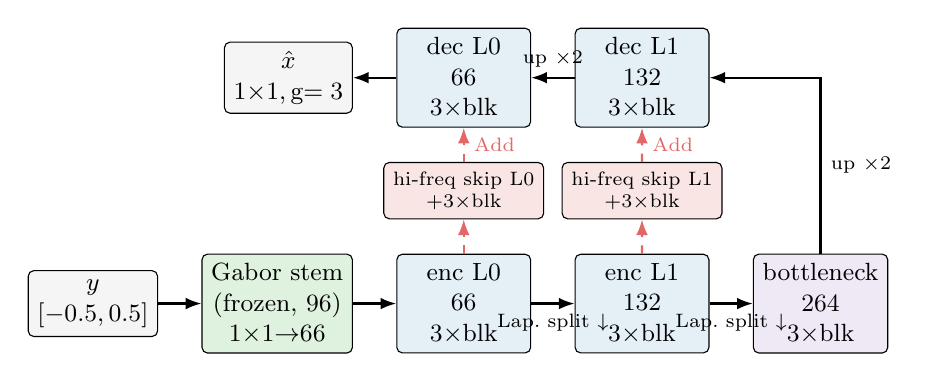
\begin{tikzpicture}[
  font=\small,
  node distance=0.55cm and 0.55cm,
  stem/.style={draw, rounded corners=2pt, minimum width=1.9cm, minimum height=0.8cm, align=center, fill=gaborgreen!15},
  enc/.style={draw, rounded corners=2pt, minimum width=1.7cm, minimum height=0.8cm, align=center, fill=oursblue!12},
  bott/.style={draw, rounded corners=2pt, minimum width=1.7cm, minimum height=0.8cm, align=center, fill=bottlepurple!15},
  skip/.style={draw, rounded corners=2pt, minimum width=1.7cm, minimum height=0.7cm, align=center, fill=skipred!12, font=\scriptsize},
  io/.style={draw, rounded corners=2pt, minimum width=1.4cm, minimum height=0.8cm, align=center, fill=black!4},
  arr/.style={-{Latex[length=2mm]}, thick},
  sarr/.style={-{Latex[length=2mm]}, thick, skipred!70, dashed},
  ]
  % bottom row: encoder path
  \node[io] (in) {$y$\\$[-0.5,0.5]$};
  \node[stem, right=of in] (gab) {Gabor stem\\(frozen, 96)\\$1{\times}1{\to}66$};
  \node[enc, right=of gab] (e0) {enc L0\\$66$\\$3\times$blk};
  \node[enc, right=of e0] (e1) {enc L1\\$132$\\$3\times$blk};
  \node[bott, right=of e1] (bn) {bottleneck\\$264$\\$3\times$blk};
  \draw[arr] (in) -- (gab);
  \draw[arr] (gab) -- (e0);
  \draw[arr] (e0) -- (e1) node[midway, below, font=\scriptsize] {Lap.\ split $\downarrow$};
  \draw[arr] (e1) -- (bn) node[midway, below, font=\scriptsize] {Lap.\ split $\downarrow$};
  % top row: decoder path
  \node[enc, above=1.6cm of e1] (d1) {dec L1\\$132$\\$3\times$blk};
  \node[enc, left=of d1] (d0) {dec L0\\$66$\\$3\times$blk};
  \node[io, left=of d0] (out) {$\hat{x}$\\$1{\times}1$,\,g$=3$};
  \draw[arr] (bn) |- (d1) node[near start, right, font=\scriptsize] {up $\times2$};
  \draw[arr] (d1) -- (d0) node[midway, above, font=\scriptsize] {up $\times2$};
  \draw[arr] (d0) -- (out);
  % skip bands (high-frequency, with high_freq blocks)
  \node[skip] (s1) at ($(e1)!0.5!(d1)$) {hi-freq skip L1\\$+3\times$blk};
  \node[skip] (s0) at ($(e0)!0.5!(d0)$) {hi-freq skip L0\\$+3\times$blk};
  \draw[sarr] (e1) -- (s1); \draw[sarr] (s1) -- (d1) node[midway,right,font=\scriptsize]{Add};
  \draw[sarr] (e0) -- (s0); \draw[sarr] (s0) -- (d0) node[midway,right,font=\scriptsize]{Add};
\end{tikzpicture}%
}
\caption{\model{} data flow (channel widths shown). A frozen Gabor stem feeds a two-level \convnext{}-V1 U-Net. Downsampling is a Laplacian-pyramid split: the low-frequency band descends (solid), the full-resolution high-frequency residual becomes the skip (dashed), passing through three extra bias-free \convnext{} blocks before a parameter-free channel-matched \texttt{Add} into the decoder. The head is a bias-free grouped $1{\times}1$ convolution (3 groups). Every operation is degree-1 homogeneous at inference.}
\label{fig:arch}
\end{figure}

\subsection{U-Net topology}
The channel widths follow $c_i = \mathrm{round}(66 \cdot 2^{\,i})$ for level $i$, giving $66 \to 132$ in the encoder, $264$ at the bottleneck, and $132 \to 66$ in the decoder. Each of the five scopes (two encoder levels, bottleneck, two decoder levels) contains three \convnext{}-V1 blocks. Upsampling is bilinear ($\times 2$). Channel counts are matched by a \emph{parameter-free} \texttt{MatchChannels} operator (zero-pad to widen, slice to narrow) rather than a learned $1{\times}1$ projection, and decoder skips are fused by addition, $\mathrm{dec} \leftarrow \mathrm{Add}(\mathrm{skip},\, \texttt{MatchChannels}(\mathrm{up}))$, not by concatenation. Both choices keep the merge exactly linear and homogeneous.

\subsection{Frozen Gabor stem}
The first learnable operation a naive CNN applies to a noisy image is a small learned convolution; here it is replaced by a \emph{fixed} oriented band-pass front end. A depthwise convolution with $32$ filters per input channel and a $7{\times}7$ kernel is initialized with a Gabor bank --- each output channel is one 2D Gabor wavelet $g(u,v)=\exp\!\big(-\tfrac{u_\theta^2+\gamma^2 v_\theta^2}{2s^2}\big)\cos\!\big(\tfrac{2\pi u_\theta}{\lambda}+\psi\big)$ at a swept orientation/frequency/phase --- and marked non-trainable, so it contributes \textbf{zero} trainable parameters and never adapts. With three input channels this emits $3\times 32 = 96$ feature maps, which a single \emph{learned} bias-free $1{\times}1$ convolution mixes down to the $66$ stem channels. The rationale is standard signal processing: an oriented multi-scale band-pass decomposition is a strong, noise-agnostic image representation that the network need not spend capacity (or risk overfitting noise) to relearn.

\subsection{Laplacian-pyramid skips and high-frequency blocks}
\label{sec:laplacian}
Instead of max-pooling, each encoder junction performs a Laplacian-pyramid split. Given the level input $z$, a fixed Gaussian blur ($5{\times}5$) and stride-2 blur-pool produce the low band $\ell = \mathrm{blurpool}(\mathrm{gauss}(z))$; the high band is the full-resolution residual $h = z - \mathrm{up}(\ell)$. The split is lossless ($\mathrm{up}(\ell)+h = z$) and channel-preserving. The low band $\ell$ descends to the next level; the high band $h$ becomes the skip connection --- but only after passing through \textbf{three} additional bias-free \convnext{}-V1 blocks (\texttt{skip\_highfreq}), applied at both encoder levels. This is a wavelet-shrinkage-style inductive bias: because Gaussian noise is spectrally flat while natural-image structure concentrates at low frequencies, forcing the decoder to reconstruct from an explicit low-band descent plus a \emph{processed} high-band residual denies it the trivial full-resolution identity-copy shortcut and matches the signal/noise spectral structure of the task.

\subsection{The \convnext{}-V1 block}
\label{sec:block}
Each block is a residual branch with call order
\[
x \;\mapsto\; x + \gamma \odot \Big[\, W_{\downarrow}\,\phi\big(\,W_{\uparrow}\,\mathrm{N}\big(\mathrm{DW}_{7\times7}\,x\big)\big)\Big],
\]
where $\mathrm{DW}_{7\times7}$ is a depthwise $7{\times}7$ convolution, $\mathrm{N}$ is the normalization (Section~\ref{sec:biasfree}), $W_{\uparrow}$ is a $1{\times}1$ expansion to $4\times$ width, $\phi$ is LeakyReLU with negative slope $0.1$ (followed by dropout $0.1$ at training time), $W_{\downarrow}$ is a $1{\times}1$ reduction, and $\gamma$ is a per-channel LayerScale multiplier (initialized $10^{-4}$, floored at $10^{-6}$). \emph{All} convolutions are bias-free. We use the V1 block rather than V2: the V2 variant inserts a Global Response Normalization whose learnable additive $\beta$ is bias-like and would break strict bias-freedom.

\subsection{Bias-free construction and degree-1 homogeneity}
\label{sec:biasfree}
The defining property of \model{} is that the entire map $D$ is positively homogeneous of degree one at inference:
\begin{equation}
D(\alpha y) = \alpha\, D(y) \qquad \text{for all } \alpha > 0.
\label{eq:homog}
\end{equation}
This holds because every constituent operation is linear-through-the-origin or degree-1 homogeneous, and no operation injects an additive constant:
\begin{itemize}
  \item every convolution (Gabor stem, $1{\times}1$ mix, all block convolutions, the head) has \texttt{use\_bias=False};
  \item the head activation is linear ($f(x)=x$);
  \item LeakyReLU is positively homogeneous, $\mathrm{LReLU}(\alpha x)=\alpha\,\mathrm{LReLU}(x)$ for $\alpha>0$ (this is why LeakyReLU is used rather than GELU, which is not homogeneous);
  \item normalization is a \emph{variance-only} batch norm, \bfbn{}: it has no running mean and no $\beta$ offset, only a fixed non-trainable running variance, so at inference $\mathrm{N}(x) = \gamma\, x / \sqrt{\mathrm{Var}+\epsilon}$ is exactly linear in $x$;
  \item the Laplacian split, \texttt{MatchChannels}, bilinear upsampling, and additive skip merge are all linear.
\end{itemize}
The choice of \bfbn{} over the \convnext{} default LayerNorm is essential and not cosmetic: LayerNorm divides by a per-sample statistic that itself scales with the input, making it scale-\emph{invariant} (degree-0), which would destroy Eq.~\eqref{eq:homog} for the whole network. We flag one scoping caveat that most treatments omit: homogeneity is an \emph{inference-time} property. During training \bfbn{} uses the per-batch variance, which makes it degree-0; Eq.~\eqref{eq:homog} holds once the running statistics are frozen.

% ============================================================================
\section{Why bias-free: Miyasawa/Tweedie, and its limits}
\label{sec:theory}

Bias-freedom is not an aesthetic choice; it is what connects the trained denoiser to a score, and what lets one blind model span a wide noise range. We state the motivation and then, in the same breath, its boundaries.

\paragraph{Miyasawa/Tweedie.}
For $y = x + \varepsilon$ with $\varepsilon \sim \mathcal{N}(0,\sigma^2 I)$ and marginal density $p_\sigma(y) = \int \mathcal{N}(y; x, \sigma^2 I)\, p(x)\, dx$, the minimum-MSE estimator obeys the Miyasawa/Tweedie identity
\begin{equation}
\hat{x}(y) \;=\; \E[x \mid y] \;=\; y + \sigma^2\, \nabla_y \log p_\sigma(y).
\label{eq:tweedie}
\end{equation}
Hence the denoiser \emph{residual} $f(y) = D(y) - y$ is, for an MMSE-optimal $D$, exactly $\sigma^2$ times the score $\nabla_y \log p_\sigma(y)$ of the noise-blurred density. Training with a plain mean-squared-error objective is therefore not an arbitrary loss: it drives $D$ toward the MMSE estimator whose residual is (a scaled) score. This is the reason \model{} is trained with MSE and read as an implicit-prior score model.

\paragraph{Homogeneity buys blind generalization.}
\citet{mohan2020biasfree} observe that a bias-free denoiser is degree-1 homogeneous (Eq.~\eqref{eq:homog}) and therefore behaves as a locally linear, input-adaptive filter $D(y) \approx J(y)\,y$ whose Jacobian $J(y)=\partial D/\partial y$ is degree-0 (scale-invariant). Because $J$ depends only on the \emph{direction} of $y$, not its magnitude, a network trained over one range of noise levels extrapolates gracefully to unseen levels --- whereas a biased network, whose additive terms fix an absolute scale, collapses off its training range. This is precisely the property that makes a single blind model viable, and the empirical target of our noise curriculum (Section~\ref{sec:protocol}).

\paragraph{What homogeneity does \emph{not} buy.}
\label{sec:theory-limits}
We are careful here, because it is easy to over-read Eq.~\eqref{eq:tweedie}. Two boundaries hold and are stated as first-class caveats:
\begin{enumerate}
  \item \textbf{Homogeneity is checkpoint-specific, not an architectural guarantee.} A network is exactly homogeneous only if it is \emph{truly} bias-free in every operation. For this checkpoint the relative homogeneity error $\lVert D(\alpha y)-\alpha D(y)\rVert / \lVert \alpha D(y)\rVert$ is at the level of floating-point round-off across $\alpha \in \{\tfrac14,\tfrac12,2,4,8\}$; but sibling checkpoints of the same family have shown deviations up to $\sim 0.14$ when a single non-homogeneous operation slips in. Eq.~\eqref{eq:homog} must be \emph{verified} per checkpoint, not assumed.
  \item \textbf{The learned residual is not a conservative field.} Eq.~\eqref{eq:tweedie} would make $f(y)$ the gradient of the scalar $\sigma^2 \log p_\sigma(y)$ only if the Jacobian $J(y)$ were symmetric. It is not: on trained checkpoints of this family the measured Jacobian asymmetry $\lVert J - J^\top\rVert / \lVert J\rVert$ is $\mathcal{O}(0.5)$ --- roughly four orders of magnitude above a symmetric-blur control --- so \textbf{no global energy/log-density function exists} whose gradient is the residual. Consequently, plug-and-play and Regularization-by-Denoising convergence guarantees (which assume a conservative, symmetric-Jacobian denoiser) do not transfer, and the residual should be read as a useful \emph{local} score estimate, not a calibrated global prior.
\end{enumerate}
We return to the practical consequences (including uncertainty calibration) in Section~\ref{sec:limitations}.

% ============================================================================
\section{Experimental protocol}
\label{sec:protocol}

\paragraph{Data and noise curriculum.}
We train on $256{\times}256$ patches drawn from COCO (\texttt{train2017}) and DIV2K (\texttt{train}), sourced with a per-directory weighting so the $\sim$118K COCO images do not drown DIV2K's $\sim$800. Patches are normalized to $[-0.5,+0.5]$ (peak-to-peak range $1.0$) and corrupted with additive Gaussian noise whose per-patch standard deviation is drawn uniformly from $[0,\, \sigma_{\max}]$, where the upper bound $\sigma_{\max}$ is widened linearly over training by a curriculum callback from $0.025$ to $0.5$ across $100$ epochs. Starting narrow and widening stabilizes early optimization; bias-freedom then supplies the cross-level generalization.

\paragraph{The $\sigma$ convention (stated precisely).}
The model operates entirely in $[-0.5,+0.5]$, so its noise level $\sigma_{\mathrm{norm}} \in [0, 0.5]$. The literature reports noise on the $[0,255]$ pixel scale; the two are related by $\sigpx = \sigma_{\mathrm{norm}} \cdot 255$. The curriculum's $\sigma_{\max}: 0.025 \to 0.5$ therefore spans $\sigpx \approx 6.4 \to 127.5$ --- it covers and exceeds the classic $15/25/50$ benchmark regimes as a single blind model. All PSNR values are computed with $\mathrm{max\_val}=1.0$ (matched to the peak-to-peak range); because PSNR is scale-invariant under a matched range, these dB numbers are directly comparable to published $\mathrm{max\_val}=255$ results, with no further conversion.

\paragraph{Optimization.}
Loss is plain MSE (the Miyasawa-optimal objective, Section~\ref{sec:theory}). We use AdamW (learning rate $10^{-3}$, cosine decay, $10$ warmup epochs, decoupled weight decay $4\times10^{-3}$), gradient-norm clipping at $1.0$, batch size $4$, $100$ epochs, full \texttt{fp32} (mixed precision was measured slower on this convolution-heavy U-Net because the bilinear-upsample gradient forces XLA off).

\paragraph{Evaluation.}
We report two evaluations of the \emph{single} trained checkpoint. (i) A blind PSNR-vs-noise sweep on DIV2K-validation ($100$ patches at $256$px). (ii) The standard leaderboard comparison on all four color sets (CBSD68, Kodak24, McMaster, Urban100) at $\sigma \in \{15,25,50\}$ using the \textbf{full-image protocol} (whole images, reflect-padded to a multiple of $16$), the same protocol the published numbers use. We additionally report a post-hoc per-pixel split-conformal coverage study. Two evaluation samples differ (100 vs.\ 32 patches for the sweep vs.\ the coverage study), so their PSNR columns are independent measurements, not cross-checks of one another.

% ============================================================================
\section{Results}
\label{sec:results}

\subsection{Blind denoising across noise levels}
Figure~\ref{fig:psnrsweep} shows the blind PSNR-vs-noise sweep on DIV2K-validation. A single model, given no noise-level input, denoises across the whole curriculum range, from $40.7$\,dB at $\sigpx{=}5$ down to $29.1$\,dB at $\sigpx{=}65$, improving the noisy input by $+6.4$ to $+15.8$\,dB.

\begin{figure}[H]
\centering
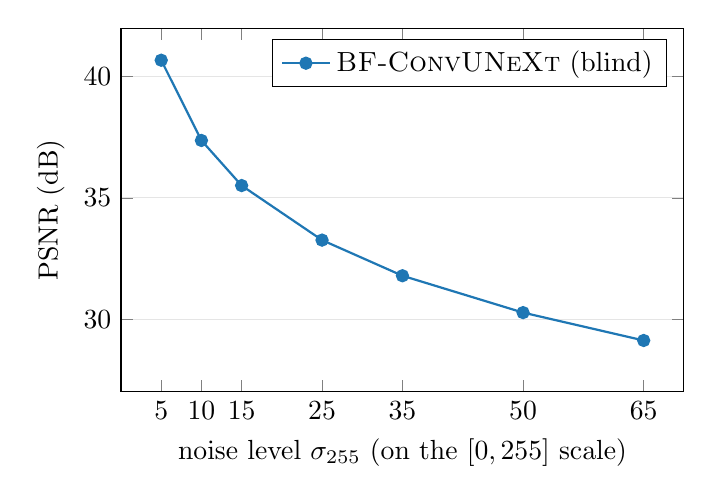
\begin{tikzpicture}
\begin{axis}[
  width=0.72\textwidth, height=6.2cm,
  xlabel={noise level $\sigpx$ (on the $[0,255]$ scale)},
  ylabel={PSNR (dB)},
  xmin=0, xmax=70, ymin=27, ymax=42,
  xtick={5,10,15,25,35,50,65},
  ymajorgrids=true, grid style={gray!20},
  legend pos=north east, legend cell align={left},
  mark size=2pt,
]
\addplot[oursblue, thick, mark=*] coordinates {
  (5,40.68) (10,37.37) (15,35.51) (25,33.26) (35,31.79) (50,30.27) (65,29.12)
};
\addlegendentry{\model{} (blind)}
\end{axis}
\end{tikzpicture}
\caption{Blind PSNR vs.\ noise on DIV2K-validation ($100$ patches, $256$px). One model spans $\sigpx \approx 5$--$65$ with no noise-level input; $95\%$ bootstrap CIs (not shown) are $\pm 0.4$--$0.8$\,dB.}
\label{fig:psnrsweep}
\end{figure}

\subsection{Comparison against the color-denoising leaderboard}
Table~\ref{tab:sota} places \model{} against six published baselines on all four standard color sets at $\sigma\in\{15,25,50\}$, under the identical full-image protocol and PSNR convention. The pattern is uniform: the single $3.39$M blind model \textbf{beats DnCNN and FFDNet on every set at every noise level}, and trails the heavyweight state of the art by a small, consistent margin that widens on Urban100.

\begin{table}[H]
\centering
\caption{Color AWGN denoising, PSNR (dB), full-image protocol. \model{} is a single $3.39$M-parameter blind model (no noise-level input). Baseline numbers are the published values collated by \citet{zhang2022scunet}. \textbf{Bold} marks where \model{} beats a given baseline. Approximate parameter counts are listed in the header; DnCNN/FFDNet are $<1$M, the four rightmost are $12$--$33$M.}
\label{tab:sota}
\renewcommand{\arraystretch}{1.12}
\resizebox{\textwidth}{!}{%
\begin{tabular}{llccccccc}
\toprule
\textbf{Set} & \textbf{$\sigpx$} & \textbf{\model{}} & \textbf{DnCNN} & \textbf{FFDNet} & \textbf{DRUNet} & \textbf{SwinIR} & \textbf{Restormer} & \textbf{SCUNet} \\
 & & \textbf{(3.4M)} & ($0.6$M) & ($0.5$M) & ($32$M) & ($12$M) & ($26$M) & ($18$M) \\
\midrule
CBSD68   & 15 & 33.95 & \textbf{33.90} & \textbf{33.87} & 34.30 & 34.42 & 34.40 & 34.40 \\
CBSD68   & 25 & 31.35 & \textbf{31.24} & \textbf{31.21} & 31.69 & 31.78 & 31.79 & 31.79 \\
CBSD68   & 50 & 28.18 & \textbf{27.95} & \textbf{27.96} & 28.51 & 28.56 & 28.60 & 28.61 \\
\midrule
Kodak24  & 15 & 34.97 & \textbf{34.60} & \textbf{34.63} & 35.31 & 35.34 & 35.47 & 35.34 \\
Kodak24  & 25 & 32.56 & \textbf{32.14} & \textbf{32.13} & 32.89 & 32.89 & 33.04 & 32.92 \\
Kodak24  & 50 & 29.51 & \textbf{28.95} & \textbf{28.98} & 29.86 & 29.79 & 30.01 & 29.87 \\
\midrule
McMaster & 15 & 34.79 & \textbf{33.45} & \textbf{34.66} & 35.40 & 35.61 & 35.61 & 35.60 \\
McMaster & 25 & 32.61 & \textbf{31.52} & \textbf{32.35} & 33.14 & 33.20 & 33.34 & 33.34 \\
McMaster & 50 & 29.61 & \textbf{28.62} & \textbf{29.18} & 30.08 & 30.22 & 30.30 & 30.29 \\
\midrule
Urban100 & 15 & 34.20 & \textbf{32.98} & \textbf{33.83} & 34.81 & 35.13 & 35.13 & 35.18 \\
Urban100 & 25 & 31.92 & \textbf{30.81} & \textbf{31.40} & 32.60 & 32.90 & 32.96 & 33.03 \\
Urban100 & 50 & 28.81 & \textbf{27.59} & \textbf{28.05} & 29.61 & 29.82 & 30.02 & 30.14 \\
\midrule
\multicolumn{2}{l}{\emph{avg} $\sigma{=}15$} & 34.48 & \textbf{33.73} & \textbf{34.25} & 34.96 & 35.13 & 35.15 & 35.13 \\
\multicolumn{2}{l}{\emph{avg} $\sigma{=}25$} & 32.11 & \textbf{31.43} & \textbf{31.77} & 32.58 & 32.69 & 32.78 & 32.77 \\
\multicolumn{2}{l}{\emph{avg} $\sigma{=}50$} & 29.03 & \textbf{28.28} & \textbf{28.54} & 29.52 & 29.60 & 29.73 & 29.73 \\
\bottomrule
\end{tabular}%
}
\end{table}

Averaged over the four sets, \model{} is $+0.75/+0.68/+0.75$\,dB above DnCNN at $\sigma=15/25/50$ and $+0.23/+0.34/+0.49$\,dB above FFDNet (which, unlike our model, is \emph{non-blind} and receives a noise-level map). It is $-0.48/-0.47/-0.49$\,dB relative to DRUNet and $-0.67/-0.67/-0.70$\,dB relative to Restormer, the leaderboard top. The gap is smallest on CBSD68/Kodak24 ($\sim0.4$\,dB), larger on McMaster ($\sim0.7$\,dB), and largest on Urban100 ($\sim1.0$\,dB) --- Urban100's repetitive, self-similar structures are exactly where the transformers' non-local attention (SwinIR, Restormer) and DRUNet's large receptive field have the most to exploit and a compact local conv U-Net the least.

\subsection{Accuracy for the parameter budget}
The point of Table~\ref{tab:sota} is not that \model{} wins outright --- it does not --- but where it sits on the accuracy/size trade-off. Figure~\ref{fig:params} plots the four-set average PSNR at $\sigma=25$ against approximate parameter count. \model{} lands between the two size classes: comfortably above the sub-1M classic CNNs it beats, and within half a dB of models $8$--$10\times$ larger.

\begin{figure}[H]
\centering
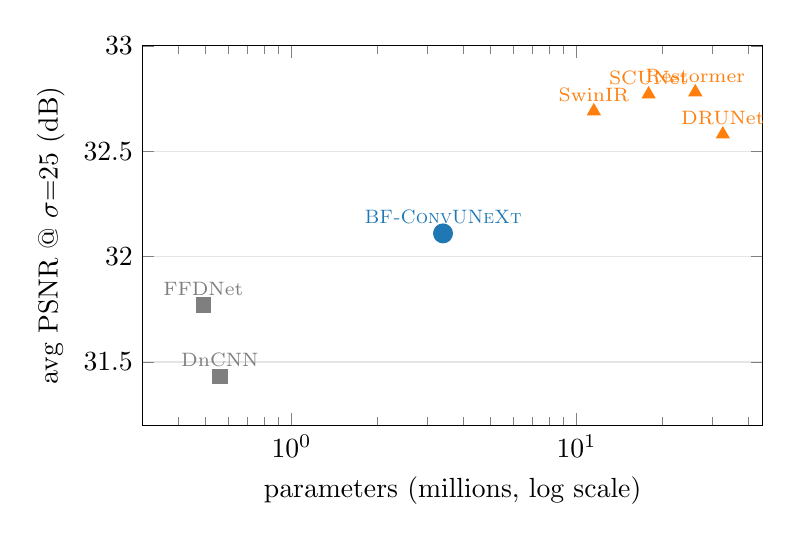
\begin{tikzpicture}
\begin{axis}[
  width=0.78\textwidth, height=6.4cm,
  xlabel={parameters (millions, log scale)},
  ylabel={avg PSNR @ $\sigma{=}25$ (dB)},
  xmode=log, log basis x=10,
  xmin=0.3, xmax=45, ymin=31.2, ymax=33.0,
  ymajorgrids=true, grid style={gray!20},
  nodes near coords, point meta=explicit symbolic,
  nodes near coords style={font=\scriptsize, anchor=south},
  only marks, mark size=2.6pt,
]
\addplot[classicgray, mark=square*] coordinates {
  (0.49,31.77) [FFDNet]
  (0.56,31.43) [DnCNN]
};
\addplot[oursblue, mark=*, mark size=3.4pt] coordinates {
  (3.4,32.11) [\model{}]
};
\addplot[sotaorange, mark=triangle*] coordinates {
  (11.5,32.69) [SwinIR]
  (17.9,32.77) [SCUNet]
  (26.1,32.78) [Restormer]
  (32.6,32.58) [DRUNet]
};
\end{axis}
\end{tikzpicture}
\caption{Four-set average PSNR at $\sigma{=}25$ vs.\ (approximate) parameter count. \model{} (blue) sits on the efficient side of the trade-off: above the sub-1M CNNs and within $\sim0.5$--$0.7$\,dB of the $12$--$33$M state of the art at $\sim1/8$--$1/10$ of their size. Parameter counts are approximate and collated from the respective papers.}
\label{fig:params}
\end{figure}

\subsection{Per-pixel uncertainty: honest coverage}
\label{sec:coverage}
Because the residual is a local score estimate, a natural question is whether a simple post-hoc interval calibrates. We ran split-conformal per-pixel intervals (per-$\sigma$ Mondrian, target coverage $0.90$, $\alpha=0.1$, $32$ calibration images) on the checkpoint; Table~\ref{tab:coverage} reports empirical coverage, mean interval width, and the matched test-split PSNR. Coverage is systematically $\sim0.877$, about $2.3$ points below the $0.90$ target.

\begin{table}[H]
\centering
\caption{Post-hoc split-conformal per-pixel coverage (target $0.90$). Coverage is systematically below target; see text for why this is expected, not a bug.}
\label{tab:coverage}
\renewcommand{\arraystretch}{1.1}
\begin{tabular}{lccc}
\toprule
$\sigma_{\mathrm{norm}}$ & empirical coverage & mean width & test PSNR (dB) \\
\midrule
0.05 & 0.877 & 0.053 & 35.08 \\
0.10 & 0.879 & 0.076 & 31.73 \\
0.15 & 0.878 & 0.093 & 29.80 \\
0.20 & 0.878 & 0.107 & 28.45 \\
0.25 & 0.877 & 0.119 & 27.38 \\
\bottomrule
\end{tabular}
\end{table}

We resist the temptation to call this finite-sample noise. With $32$ images the calibration pool is $\sim 6.3$M pixels, so the conformal quantile is estimated essentially exactly; a well-specified split conformal would sit at $0.90$. The systematic $\sim0.877$ instead reflects a genuine exchangeability gap: a \emph{single} per-$\sigma$ quantile pools pixels across images whose per-image residual scales are heterogeneous, so pixel-level exchangeability requires image-level exchangeability, which does not fully hold on held-out images. Image-conditional or variance-scaled conformal would tighten it; that is out of scope here. We report it because a paper that shows the coverage table but hides the undercoverage would be dishonest.

% ============================================================================
\section{Discussion: limitations and what does not work}
\label{sec:limitations}

\paragraph{Where it wins, and where it does not.}
\model{} is a strong \emph{compact, blind} denoiser: it beats the classic sub-1M CNNs everywhere and closes most of the gap to models an order of magnitude larger, from a single checkpoint with no noise-level input. It does \emph{not} beat the heavyweight state of the art, and the gap is structurally largest on Urban100, where non-local self-similarity rewards attention and large receptive fields that a two-level local conv U-Net lacks. We do not claim otherwise.

\paragraph{The theory's limits are real, not rhetorical.}
As shown in Section~\ref{sec:theory-limits}, the learned residual field is measurably non-conservative, so \model{} does \emph{not} define a global image prior, an exact likelihood, or a calibrated posterior. Uses that require a conservative denoiser --- provable plug-and-play/RED convergence, energy-based sampling with a fixed target, calibrated Bayesian uncertainty --- are outside what this model licenses, and the undercoverage in Section~\ref{sec:coverage} is a concrete downstream symptom. The homogeneity that does hold is inference-only and must be re-verified per checkpoint rather than assumed from the architecture.

\paragraph{Measurement limits.}
We report \textbf{PSNR only}; SSIM was not measured and no SSIM number appears in this paper. All results are from a \textbf{single checkpoint} --- there is no multi-seed variance estimate --- and we present \textbf{no ablations}: the individual contributions of the frozen Gabor stem, the Laplacian high-frequency skips, the \texttt{high\_freq\_blocks}, the bias-free normalization, and the noise curriculum are \emph{not} isolated here. CBSD68 and McMaster are the two standard color sets we could evaluate on locally alongside Kodak24 and Urban100; grayscale Set12/BSD68 would require a one-channel model. Each of these is deliberate scope, and each is the obvious next experiment.

\paragraph{Future work.}
The natural follow-ups are (i) a controlled ablation isolating each component's dB contribution with multi-seed variance; (ii) SSIM and a perceptual metric alongside PSNR; (iii) larger-capacity and deeper variants to probe how much of the SOTA gap is capacity vs.\ architecture; and (iv) a study of whether a symmetrized or explicitly conservative variant recovers the plug-and-play guarantees the current model forgoes, and at what accuracy cost.

% ============================================================================
\section{Related work}
\label{sec:related}

\paragraph{Bias-free denoising.}
\citet{mohan2020biasfree} introduced bias-free CNNs for blind denoising and established the degree-1-homogeneity argument we build on. The residual-as-score reading rests on the classical Miyasawa/Tweedie identity \citep{miyasawa1961,robbins1956}, which also underpins the implicit-prior sampling line of \citet{kadkhodaie2021stochastic}. \model{} applies the bias-free discipline end-to-end to a modern block and front end.

\paragraph{CNN and transformer denoisers.}
DnCNN \citep{zhang2017dncnn} established the residual-CNN denoiser; FFDNet \citep{zhang2018ffdnet} added a noise-level map for non-blind flexibility; DRUNet \citep{zhang2021plugandplay} coupled a U-Net denoiser with plug-and-play restoration; SwinIR \citep{liang2021swinir}, Restormer \citep{zamir2022restormer}, and SCUNet \citep{zhang2022scunet} brought (windowed/channel) attention and are the current leaderboard leaders. These are our baselines; all except our model and DnCNN's blind variant either use a noise map or are larger by $8$--$60\times$.

\paragraph{Building blocks.}
The block is a \convnext{} \citep{liu2022convnext} in a U-Net \citep{ronneberger2015unet}. The multi-scale skip decomposition is a Laplacian pyramid \citep{burt1983laplacian}, and the frozen front end is a Gabor filter bank \citep{gabor1946}. \model{} contributes their bias-preserving integration and its measurement, not the pieces.

% ============================================================================
\section{Reproducibility}
\label{sec:repro}

The evaluated checkpoint is \texttt{convunext\_denoiser\_base} ($3{,}393{,}936$ parameters; depth $2$; widths $66/132/264$; three \convnext{}-V1 blocks per scope plus three per high-frequency skip band; frozen $32$-filter, $7{\times}7$ Gabor stem; \bfbn{}; LeakyReLU($0.1$); linear grouped head). It was trained with the recipe of Section~\ref{sec:protocol}. The full-image benchmark uses whole test images reflect-padded to a multiple of $16$, PSNR at $\mathrm{max\_val}=1.0$ on $[-0.5,0.5]$, on the standard CBSD68 / Kodak24 / McMaster / Urban100 sets. All numbers in Table~\ref{tab:sota}, Table~\ref{tab:coverage}, and Figure~\ref{fig:psnrsweep} are measured from that single checkpoint; baseline numbers are the published values as collated by \citet{zhang2022scunet}.

% ============================================================================
\section{Conclusion}
\label{sec:conclusion}

We described \model{}, a compact bias-free \convnext{} U-Net that integrates a frozen Gabor stem, Laplacian-pyramid high-frequency skips, and end-to-end degree-1 homogeneity, and we measured it honestly against the color-denoising leaderboard. As a single $3.4$M-parameter blind model it beats the classic sub-1M CNNs on all four standard sets at all three noise levels and comes within about half a dB of state-of-the-art models an order of magnitude larger, with the residual gap concentrated on self-similar imagery. We were equally explicit about the boundaries: the bias-free homogeneity is inference-only and checkpoint-specific, the learned operator is non-conservative and thus not a global prior, and we report a single checkpoint on PSNR without ablations. The contribution is a clean, reproducible integration and a fair benchmark, not a novelty claim --- and, we hope, a useful data point on how much of modern denoising accuracy is reachable from a small, strictly bias-free model.

% ============================================================================
\bibliographystyle{plainnat}
\begin{thebibliography}{99}

\bibitem[Burt \& Adelson(1983)]{burt1983laplacian}
Burt, P.~J., \& Adelson, E.~H. (1983).
\newblock The Laplacian pyramid as a compact image code.
\newblock \emph{IEEE Transactions on Communications}, 31(4), 532--540.

\bibitem[Gabor(1946)]{gabor1946}
Gabor, D. (1946).
\newblock Theory of communication.
\newblock \emph{Journal of the Institution of Electrical Engineers}, 93(26), 429--457.

\bibitem[Kadkhodaie \& Simoncelli(2021)]{kadkhodaie2021stochastic}
Kadkhodaie, Z., \& Simoncelli, E.~P. (2021).
\newblock Stochastic solutions for linear inverse problems using the prior implicit in a denoiser.
\newblock \emph{Advances in Neural Information Processing Systems (NeurIPS)}. arXiv:2007.13640.

\bibitem[Liang et al.(2021)]{liang2021swinir}
Liang, J., Cao, J., Sun, G., Zhang, K., Van Gool, L., \& Timofte, R. (2021).
\newblock SwinIR: Image restoration using Swin Transformer.
\newblock \emph{ICCV Workshops}. arXiv:2108.10257.

\bibitem[Liu et al.(2022)]{liu2022convnext}
Liu, Z., Mao, H., Wu, C.-Y., Feichtenhofer, C., Darrell, T., \& Xie, S. (2022).
\newblock A ConvNet for the 2020s.
\newblock \emph{CVPR}. arXiv:2201.03545.

\bibitem[Miyasawa(1961)]{miyasawa1961}
Miyasawa, K. (1961).
\newblock An empirical Bayes estimator of the mean of a normal population.
\newblock \emph{Bulletin of the International Statistical Institute}, 38(4), 181--188.

\bibitem[Mohan et al.(2020)]{mohan2020biasfree}
Mohan, S., Kadkhodaie, Z., Simoncelli, E.~P., \& Fernandez-Granda, C. (2020).
\newblock Robust and interpretable blind image denoising via bias-free convolutional neural networks.
\newblock \emph{International Conference on Learning Representations (ICLR)}. arXiv:1906.05478.

\bibitem[Robbins(1956)]{robbins1956}
Robbins, H. (1956).
\newblock An empirical Bayes approach to statistics.
\newblock \emph{Proceedings of the Third Berkeley Symposium on Mathematical Statistics and Probability}, 1, 157--163.

\bibitem[Ronneberger et al.(2015)]{ronneberger2015unet}
Ronneberger, O., Fischer, P., \& Brox, T. (2015).
\newblock U-Net: Convolutional networks for biomedical image segmentation.
\newblock \emph{MICCAI}. arXiv:1505.04597.

\bibitem[Zamir et al.(2022)]{zamir2022restormer}
Zamir, S.~W., Arora, A., Khan, S., Hayat, M., Khan, F.~S., \& Yang, M.-H. (2022).
\newblock Restormer: Efficient transformer for high-resolution image restoration.
\newblock \emph{CVPR}. arXiv:2111.09881.

\bibitem[Zhang et al.(2017)]{zhang2017dncnn}
Zhang, K., Zuo, W., Chen, Y., Meng, D., \& Zhang, L. (2017).
\newblock Beyond a Gaussian denoiser: Residual learning of deep CNN for image denoising.
\newblock \emph{IEEE Transactions on Image Processing}, 26(7), 3142--3155. arXiv:1608.03981.

\bibitem[Zhang et al.(2018)]{zhang2018ffdnet}
Zhang, K., Zuo, W., \& Zhang, L. (2018).
\newblock FFDNet: Toward a fast and flexible solution for CNN-based image denoising.
\newblock \emph{IEEE Transactions on Image Processing}, 27(9), 4608--4622. arXiv:1710.04026.

\bibitem[Zhang et al.(2021)]{zhang2021plugandplay}
Zhang, K., Li, Y., Zuo, W., Zhang, L., Van Gool, L., \& Timofte, R. (2021).
\newblock Plug-and-play image restoration with deep denoiser prior.
\newblock \emph{IEEE Transactions on Pattern Analysis and Machine Intelligence}, 44(10), 6360--6376. arXiv:2008.13751.

\bibitem[Zhang et al.(2022)]{zhang2022scunet}
Zhang, K., Li, Y., Liang, J., Cao, J., Zhang, Y., Tang, H., Fan, D.-P., Timofte, R., \& Van Gool, L. (2022).
\newblock Practical blind image denoising via Swin-Conv-UNet and data synthesis.
\newblock arXiv:2203.13278.

\end{thebibliography}

\end{document}
